% -*- coding: utf-8 -*-
%%%%%%%%%%%%%%%%%%%%%%%%%%%%%%%%%%%%%%%%%%%%%%%%%%%%%%%%%%%%%%%%%%%%%%%%%%%%%%%%
%2345678901234567890123456789012345678901234567890123456789012345678901234567890
%        1         2         3         4         5         6         7         8

%\UseRawInputEncoding


\documentclass[letterpaper, 10 pt, conference]{ieeeconf}  % Comment this line out if you need a4paper

%\pdfminorversion=4              % tell pdflatex to generate PDF in version 1.4
\usepackage[T1]{fontenc}
\usepackage{cite}
\usepackage{amssymb,amsfonts}
\usepackage{algorithmic}
\usepackage{graphicx}
\usepackage{textcomp}
\usepackage{changes}
\usepackage{subcaption}
\usepackage{xcolor}
\usepackage{color, soul}
\usepackage{amsmath}
\usepackage{booktabs}
\usepackage{multirow}
\usepackage{xstring}
%\documentclass[a4paper, 10pt, conference]{ieeeconf}      % Use this line for a4 paper

\IEEEoverridecommandlockouts                              % This command is only needed if 
                                                          % you want to use the \thanks command

\overrideIEEEmargins                                      % Needed to meet printer requirements.

%In case you encounter the following error:
%Error 1010 The PDF file may be corrupt (unable to open PDF file) OR
%Error 1000 An error occurred while parsing a contents stream. Unable to analyze the PDF file.
%This is a known problem with pdfLaTeX conversion filter. The file cannot be opened with acrobat reader
%Please use one of the alternatives below to circumvent this error by uncommenting one or the other
%\pdfobjcompresslevel=0
%\pdfminorversion=4

% See the \addtolength command later in the file to balance the column lengths
% on the last page of the document

% The following packages can be found on http:\\www.ctan.org
%\usepackage{graphics} % for pdf, bitmapped graphics files
%\usepackage{epsfig} % for postscript graphics files
%\usepackage{mathptmx} % assumes new font selection scheme installed
%\usepackage{times} % assumes new font selection scheme installed
%\usepackage{amsmath} % assumes amsmath package installed
%\usepackage{amssymb}  % assumes amsmath package installed
\usepackage{cite}

\title{\LARGE \bf
RONet: Real-time Range-only Indoor Localization via Stacked Bidirectional LSTM with Residual Attention}


\author{Hyungtae Lim$^{1}$ , Changgyu Park$^{2}$, Hyun Myung$^{3}$, \textit{Senior Member, IEEE}% <-this % stops a space
\thanks{
	*This material is based upon work supported by the Ministry of Trade, Industry \& Energy(MOTIE, Korea) under Industrial Technology Innovation Program. No.10067202, 'Development of Disaster Response Robot System for Lifesaving and Supporting Fire Fighters at Complex Disaster Environment'.}% <-this % stops a space
\thanks{$^{1}$Hyungtae Lim, $^{2}$Jungmo Koo, $^{3}$Jieum Hyun, and $^{4}$Hyun Myung are with
	the Urban Robotics Laboratory, Korea Advanced Institute of Science
	and Technology (KAIST) Daejeon, 34141, South Korea. {\tt\small \{shapelim, jungmokoo, jimi, hmyung\}@kaist.ac.kr}}%
%
}


\begin{document}

\captionsetup[figure]{labelformat={default},labelsep=period,name={Fig.}}


\maketitle
\thispagestyle{empty}
\pagestyle{empty}


%%%%%%%%%%%%%%%%%%%%%%%%%%%%%%%%%%%%%%%%%%%%%%%%%%%%%%%%%%%%%%%%%%%%%%%%%%%%%%%%
\begin{abstract}



Range-only SLAM is a method for localizing a mobile robot and beacons by mainly utilizing distance measurements. Unlike the traditional probability-based range-only SLAM method, we present a novel approach using a recurrent neural network architecture that directly learns the end-to-end mapping between distance data and robot position.
!!!
Range-only(RO) SLAM is a method for localizing a mobile robot and beacons by mainly utilizing distance measurements. Because range-only measurements have only magnitude so it has rank-deficiency. And distance is only measured by the \textcolor{red}{time of flight(TOF)}, data is noisy.

In this paper, we proposed a novel approach to range-only SLAM using multimodal bidirectional stacked LSTM models. Unlike the traditional probability-based range-only SLAM method, we present a novel approach using a recurrent neural network architecture that directly learns the end-to-end mapping between distance data and robot position.

We gathered our own dataset and tested in 2 cases exploiting eagle eye motion capturer camera. The multimodal bidirectional stacked LSTM structure exhibits the precise estimates of robot positions, but one case, it is less accurate than traditional SLAM algorithm. 
!!!!

As verified experimentally, this new proposal represents a significant improvement in accuracy, computation time, and robustness against outliers.

\end{abstract}


%%%%%%%%%%%%%%%%%%%%%%%%%%%%%%%%%%%%%%%%%%%%%%%%%%%%%%%%%%%%%%%%%%%%%%%%%%%%%%%%
\section{INTRODUCTION}

 In recent years, advancement in micro-electo-mechanical systems(MEMS) contributes the improvement of sensors' performance and miniaturization at the same time in such a way as to have enabled the industiral robots to have mobility. Accordingly, studies about techniques for localizing a mobile robot and recognizing surrounding environments, called Simultaneous Localization and Mapping(SLAM)\cite{dissanayake2001solution}, become more important and has been conducted actively. Specifically, Range-only SLAM(RO-SLAM) have addressed the problem of SLAM with a set of range-only measurements between a mobile robot and landmarks obtained from range sensors such as UWB, ultrasonic, laser-based beacon sensors. By virtue of this low-cost, small-size, acceptively accurate performance, and convenience of being installed, RO-SLAM have been suggested as a solution for localization on the indoor environment\cite{peneda2009trilateration, jung2011indoor} where the signals of the Global Positioning Systems(GPS) cannot be received, e.g., indoor environment\cite{peneda2009trilateration, jung2011indoor,raghavan2010accurate} and underwater environment\cite{newman2003pure, olson2006robust}
 
 
 The range measurements are usually measured by Time-of-Flight(TOF) and only consist of single value to represent distance between each landmark and mobile robot respectively. This cause two problems: one is that it is very vulnerable to noise because the distance are measured by only one-dimensionl information and the other one is \textit{rank dificiency} problem\cite{fabresse2018efficient}. In other words, the single value to represent distance between each landmark and mobile robot respectively is deficient to describe exact position or orientation of the landmark. Besides, these measurements could have huge uncertainties caused by multipath fading channel(MPF) problem\cite{li2017novel} in real world. To alleviate these issues, many studies based on Kalman Filter(KF) algorithm or probabilistic approaches are conducted how to estimate state of the mobile robot and landmarks more precisely with covering the uncertainties. 

\begin{figure}[h]
	
	\centering
	%\subfigure[]{
	%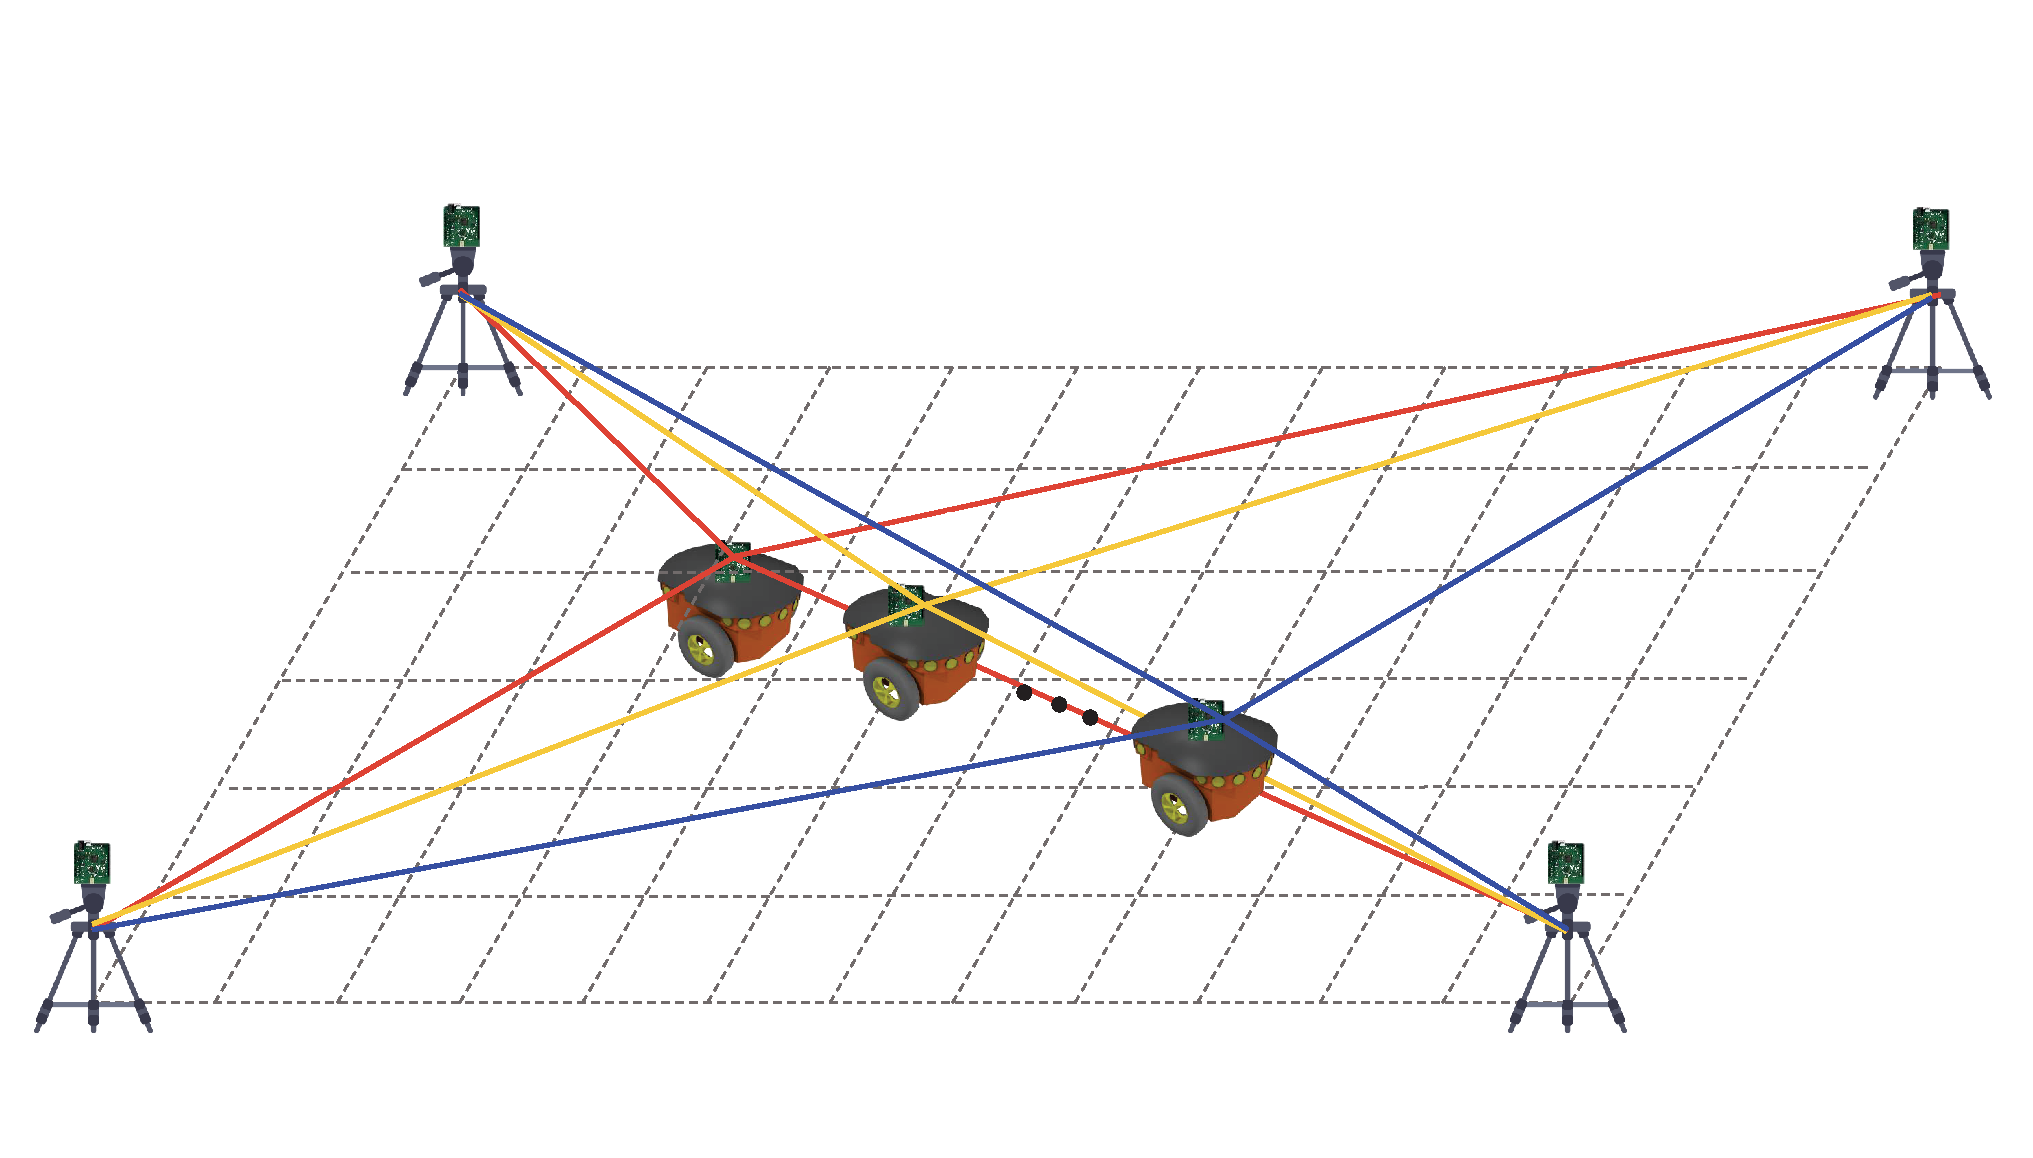
\includegraphics[height=4.5cm]{IROS2018_image_1}
	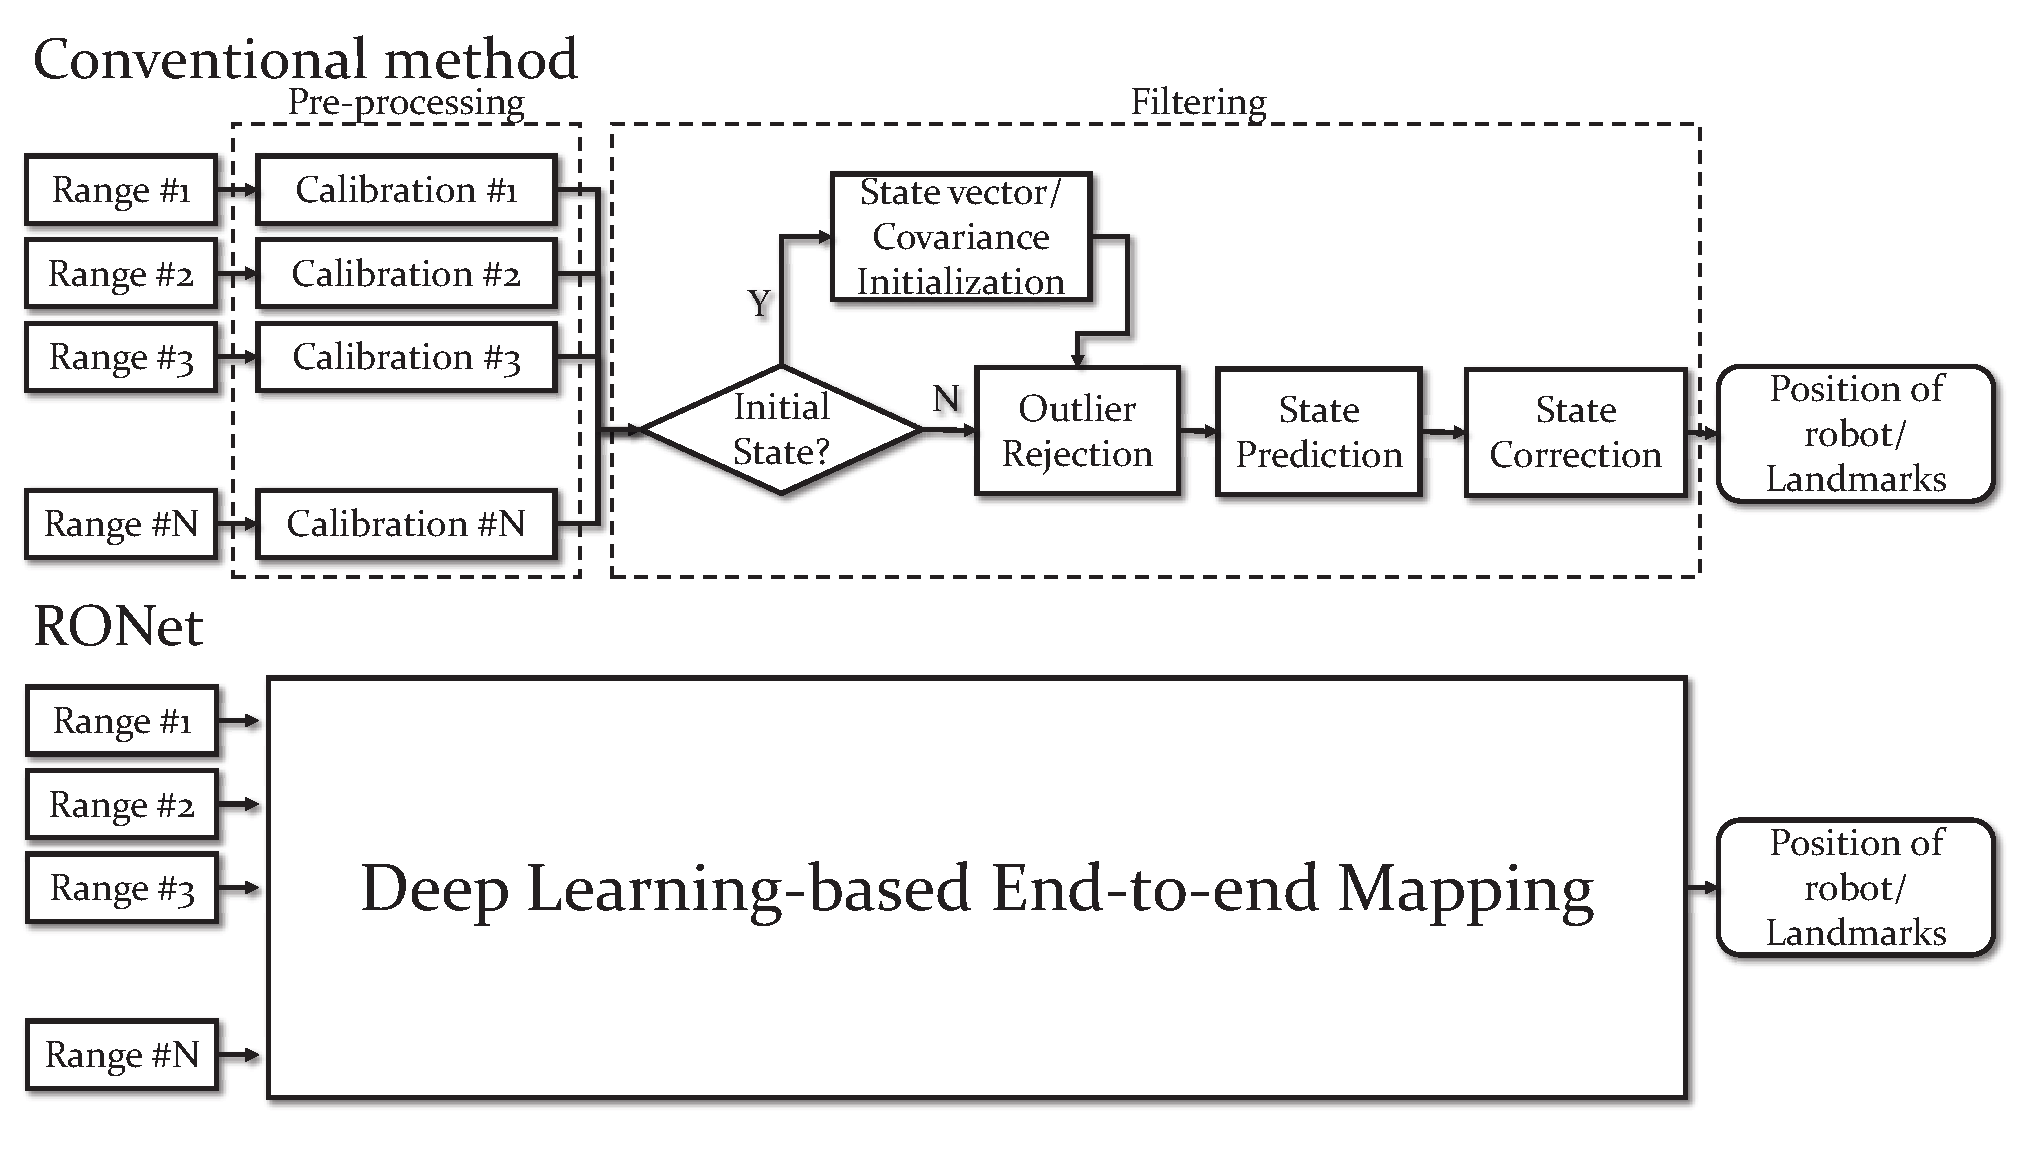
\includegraphics[height=5cm]{image/conventional_deep_comparsion}
	
	%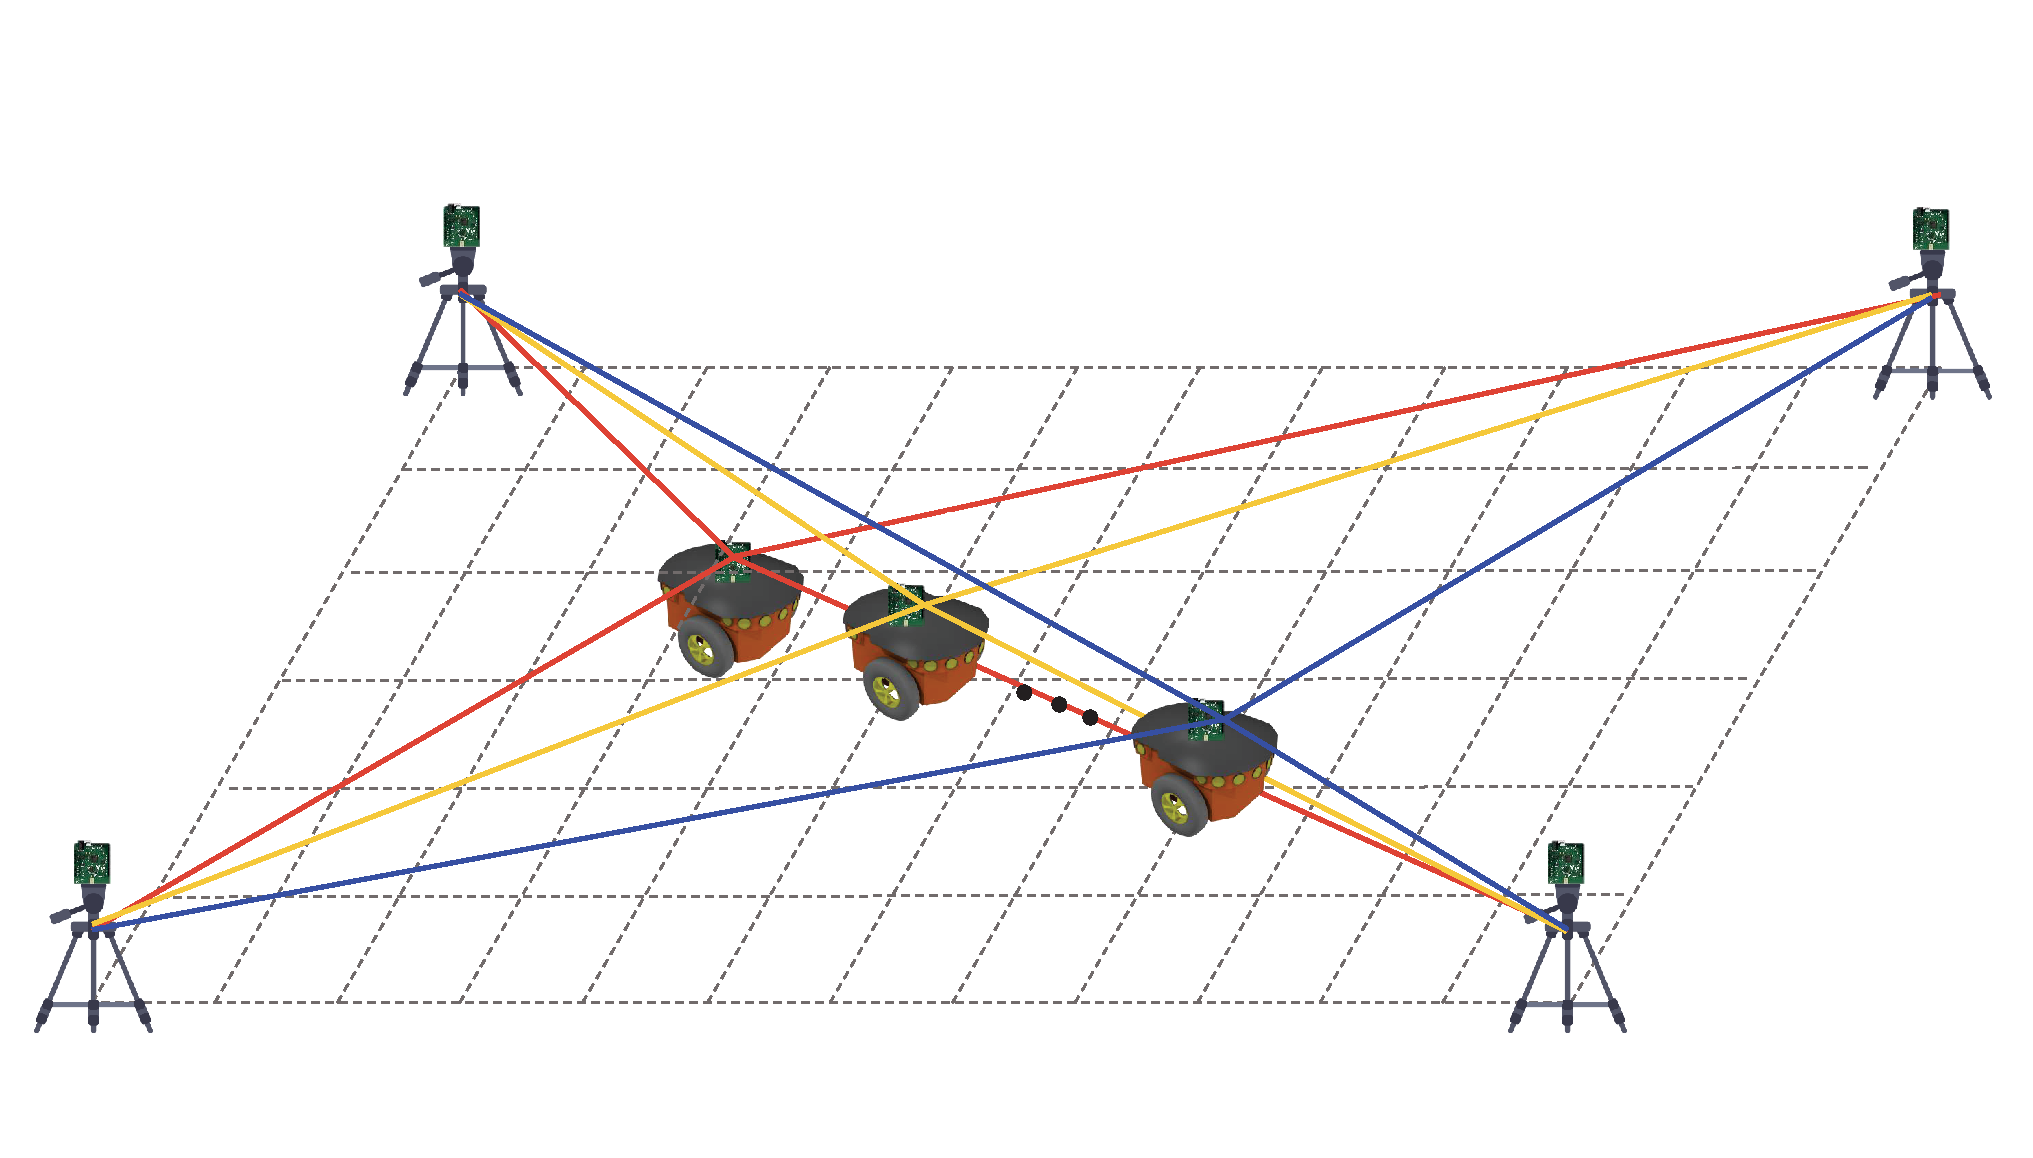
\includegraphics[trim={0 0 0 1cm}height=4.5cm]{IROS2018_image_1}
	\label{fig:example}
	%	}
	
	\caption{Comparison between a standard range-only localization or SLAM framework and our learning-based approach.}
	
\end{figure}

In this paper, we propose a robust stacked bidirectional Long Short-Term Memory(stacked Bi-LSTM) with residual attention for more accurate localization of the robot. To the best of our knowledge, it is a first approach to apply LSTM-based architecture to localize the mobile robot on the real-world in real-time using range-only measurement. Since it is achieved in an end-to-end mapping between range measurement and robot position, it does not need any preprocessing module used in the conventional RO-SLAM or range-only localization, such as an calibration and outlier rejection. Our contribution is threefold as follows:

 Using LSTM-based architecture, our structure directly learns the end-to-end mapping between range measurements and robot position. This operation non-linearly maps the relationship not only considering the long-range dependence of sequential distance data by the LSTM, but also using the correlation of the backward information and the forward information of the sequence of each time step by virtue of its bidirectional architecture. \textcolor{red}{Existing RO SLAM needs calibration before filtering, and then, range measurement undergoes outlier rejection, prediction and correction processes are needed.	Furthermorme, it uses low dimensional data to perform localization, there is a disadvantage that estimation is difficult even if the value deviates slightly from the model.} \textcolor{green}{Therefore, we solve this complex algorithm with end-to-end based deep learning. This system overview is shown in the figure below.}

\begin{itemize}
	%\setlength{\itemindent}{-.5in}
	\item Our structure directly learns the end-to-end mapping between sequential range measurements and robot position. Robust with minimal range sensors.
	\item Using neural networks, performance is higher than traditional method.
	\item Real-time on the real world
	 
\end{itemize}

The rest of the paper is organized as follows: Section II overviews the related works. Section III describes our neural network in detail and defines the problem to be considered, and Section IV describes the experimental results. Finally, Section V summarizes our contributions and points to future work.


\cite{lim2018effective}
!!!!
In the meantime, as deep learning age has come\cite{lecun2015deep},

In this paper, we propose a stacked bidirectional Long Short-Term Memory(stacked Bi-LSTM) with residual attention for more accurate localization of a MN. Our contributions can be summarized as follows. First of all, Using deep learning, our structure directly learns the end-to-end mapping between range data measured by ANs-to-MN distances and the position of MN on three dimensional space. Unlike other approaches whose authors implement MLP-based neural networks, we exploit LSTM architecture in such a way as not only to take present range data but also take previous temporal data as input for estimating the MN's position. Second, we verify that effect of the residual attention in the way that the residual attention layer makes the network better understand context of the feature when dealing with low-dimensional input. Finally, we implement the networks presented at related works and compare which neural architecture perperforms better when real-world data are given as input. As a result, and our networks perform the best performance among other proposed approaches. Our system overview is shown in the figure 


\section{Related Works}
\subsection{Conventional RO SLAM}

has been widely incorporated into robotics fields, especially utilized in the indoor environment to estimate the position of an object by distance measurements obtained from range sensors such as UWB, ultrasonic, laser-based beacon sensors \cite{thomas2005revisiting, cho2010mobile,raghavan2010accurate} due to the convenience of trilateration that estimates the position of a receiver of range sensors if one only knows range measurement. For that reasons, range-only Simultaneous Localization and Mapping(RO-SLAM) methods are utilized popularly, which not only estimate the position of the receiver of range sensors, but also localize the position of range sensors regarded as features on a map, and studies have been conducted continuously in terms of probability-based approach\cite{blanco2008pure,blanco2008efficient,fabresse2013undelayed, shetty2018particle}. communicate with other wiresless sensors efficiently and conveniently. 

In the past few years, researchers have conducted the studies using machine learning-based approaches to reduce computational complexity and localize a mobile node more precisely. One authors utilized support vector machine(SVM) for localizaiton, \cite{tran2008localization, huan2010three, feng2012determination, afzal2014localization}, other author developed method support vector regression(SVR) for localiztion\cite{lee2013new, lee2013novel}. In \cite{tran2008localization}, authors suggested two SVMs for localization, called LSVMs, one LSVM infers x-dimension and the other LSVM infers y-dimension. To employeeing LSVMs, they divide the field into \textit{M-l} x-classes and \textit{M-l} y-classes, like grid, and this deployment has had an impact on succeeding studies\cite{chatterjee2010fletcher, feng2012determination, afzal2014localization}. Samadian \textit{et al.}\cite{samadian2011probabilistic} introduced probablistic support vector machine for localization and they showed that probablistic vector machine has better performance than LSVM. In terms of SVR, Lee \textit{et al.} suggested various types of SVR for localization\cite{lee2013new, lee2013novel}  

Especially, several works have been studied using neural networks to localize nodes of the range measurement sensors on the indoor space while covering range measurements' uncertainties. Regarding previous proposals, Chenna \textit{et al.} first shows the suitability that Kalman filter could be replaced with the RNN when estimating states and tracking nodes\cite{chenna2004state}. However, they did not provide numerical analysis, so Shareef \textit{et al.} did and conducted their experiment in the real-world. They concluded Radial Basis Function(RBF) may be the best option among the suggested Kalman filter models and RNN\cite{shareef2008localization}. 

\subsection{Deep Learning and LSTM-based Sequential Modeling}

As deep learning age has come\cite{lecun2015deep}, various kinds of deep neural architectures have been proposed for many tasks related to robotics field. Especially, recurrent neural networks (RNNs), originated from Natural Language Process(NLP) area\cite{elman1990finding}, have been shown to achieve better performance in case of dealing with time variant information, thereby RNNs are widely utilized such as not only speech recognition, but also pose estimation and localization\cite{walch2017image, gladh2016deep, wang2017deepvo, kendall2015posenet, turan2018deep}. 

\subsection{Deep Learning for Low-dimensional Sensor Data}


WSNs fields also have introduced various kinds of neural network architectures\cite{rahman2009localization, singh2013tdoa, abdelhadi2013efficient, kumar2016localization, banihashemian2018new}. An main advantage of neural networks-based approaches is that the neural networks enables themselves to recognize the position of the MNs quite accurately through the training even if there is no mathematical description. The neural networks also cover all noises that occurs when ANs and MNs interchange their signals. The authors show that their nerual networks-based approach have better performance than traditional approaches or machine learning-based approaches, yet most networks are based on The Multilayer Perceptron(MLP). In addition, the some authors just show the feasibility of their approaches, i.e., they trained and tested on the simulations situation. Plus, some authors let the neural networks infer the estimates on the two-dimensional space, but gap of the complexity of estimating position between on two-dimensional space and on three-dimensional using \textit{rank-deficient} measurements cannot be negligible.
 

\begin{table*}[ht]
	\centering
	\caption{Comparison of previous studies with our approach}
	\begin{tabular}{l|l|l|l|l|l}
		\toprule
		\multicolumn{1}{c}{\textbf{Localization method}} & \multicolumn{1}{c}{\textbf{Dimension}} & \multicolumn{1}{c}{\textbf{Type of input}} & \multicolumn{1}{c}{\textbf{Train data}} & \multicolumn{1}{c}{\textbf{Test data mobility}} & \multicolumn{1}{c}{\textbf{Implementation environment}} \\ 
		\midrule
		RBF\cite{shareef2008localization}                          & \multicolumn{1}{c}{2D}                 & \multicolumn{1}{c}{Temporary}                        & \multicolumn{1}{c}{Grid}                & 
		\multicolumn{1}{c}{Dynamic nodes \checkmark}                & \multicolumn{1}{c}{Real-world \checkmark}                          \\ 
		MLP\cite{rahman2009localization}&        \multicolumn{1}{c}{2D}              &      \multicolumn{1}{c}{Temporary}                                            &   \multicolumn{1}{c}{Grid}                      & \multicolumn{1}{c}{Static nodes}                     &   \multicolumn{1}{c}{Simulation}    \\ 
		
		MLBPN\cite{singh2013tdoa}&
		\multicolumn{1}{c}{2D}                   &      
		\multicolumn{1}{c}{Temporary}                 &   \multicolumn{1}{c}{Grid}                   & 
		\multicolumn{1}{c}{Static nodes}        &   \multicolumn{1}{c}{Simulation}   \\ 
		
		MLP\cite{abdelhadi2013efficient}& 
		\multicolumn{1}{c}{3D  \checkmark}                   &      
		\multicolumn{1}{c}{Temporary}                 &   \multicolumn{1}{c}{Spread \checkmark}                   & 
		\multicolumn{1}{c}{Static nodes}        &   \multicolumn{1}{c}{Simulation}   \\ 
		
		c-FCNNs\cite{bernas2015fully}& 
		\multicolumn{1}{c}{2D}                   &      
		\multicolumn{1}{c}{Temporary}                 &   \multicolumn{1}{c}{Spread \checkmark}                   & 
		\multicolumn{1}{c}{Static nodes}        &   \multicolumn{1}{c}{Real-world  \checkmark}   \\ 
		
		MLP\cite{kumar2016localization}& 
		\multicolumn{1}{c}{2D}                   &      
		\multicolumn{1}{c}{Temporary}                 &   \multicolumn{1}{c}{Grid}                   & 
		\multicolumn{1}{c}{Static nodes}        &   \multicolumn{1}{c}{Real-world  \checkmark}   \\ 
		LPSONN\cite{banihashemian2018new}&     
		\multicolumn{1}{c}{2D}                   &      
		\multicolumn{1}{c}{Temporary}                 &   \multicolumn{1}{c}{Spread  \checkmark}                   & 
		\multicolumn{1}{c}{Static nodes}        &   \multicolumn{1}{c}{Simulation}   \\ 
		
		Ours&
		\multicolumn{1}{c}{3D \checkmark}                   &      
		\multicolumn{1}{c}{Sequential \checkmark}                 &   \multicolumn{1}{c}{Spread \checkmark}                   & 
		\multicolumn{1}{c}{Dynamic nodes \checkmark}        &   \multicolumn{1}{c}{Real-world \checkmark}   \\ 
		\bottomrule
	\end{tabular}
	\label{table:related_worsk}
	
\end{table*}

%\begin{figure*}[h]
%	\centering
%	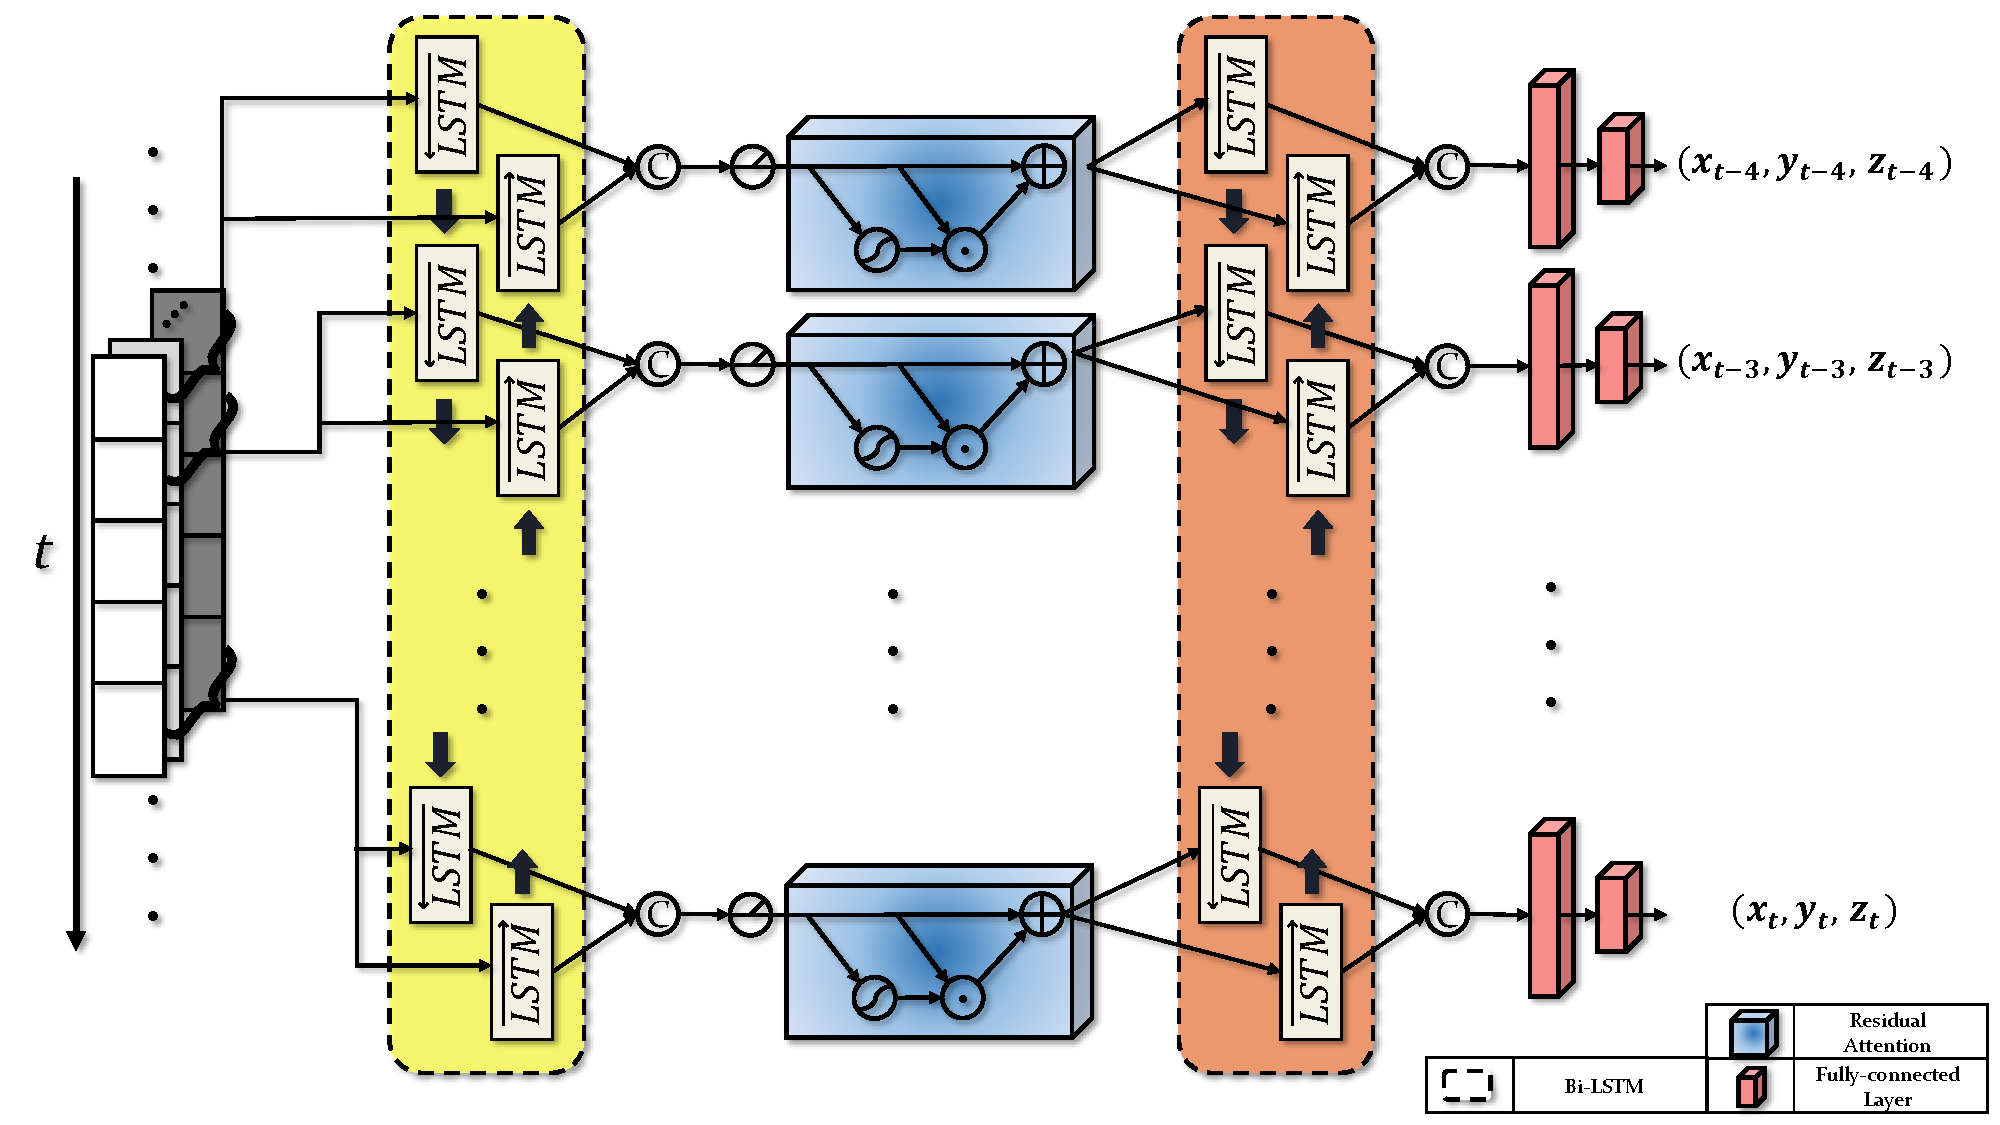
\includegraphics[width=.9\textwidth]{image/networks}
%	\caption{Our proposed network architecture.}
%	\label{fig:our_network}
%\end{figure*}

Similarly, many researchers also have achived considerable improvement to localize position of mobile node by exploiting MLP in WSNs fields\cite{shareef2008localization, rahman2009localization, singh2013tdoa,abdelhadi2013efficient,bernas2015fully, kumar2016localization, banihashemian2018new}. In case of range-based method, Rahman \textit{et al.} \cite{rahman2009localization} have considered the neural networks for mapping between RSS and corresponding position of sensor nodes and let neural networks be trained by the train data gathered by the sensor nodes that are eqaully spaced over x-axis and y-axis. In \cite{singh2013tdoa}, Singh \textit{et al.} compared that performance of Multilayer Back propagation Network Model(MLBPN) and Radial Basis Function Network Model(RBFN) and the authors show that RBFN performs better than MLBPN when the number of the sensor nodes is larger than 220. Abdelhadi \textit{et al.}  \cite{abdelhadi2013efficient} presented two artificial intelligence techniques: Sugeno-type fuzzy system and neural networks system. In addition, the authors conducted experiment on three-dimensional space in such a way as verified the feasibility of localization by utilizing nueral networks in 3D space. Kumar \textit{et al.} \cite{kumar2016localization} also introduced the neural networks and evaluated five different training techniques,e.g., Levenberg-Marquardt (LM), Bayesian Regularization
(BR), Resilient Back-propagation (RP), Scaled Conjugate Gradient (SCG) and Gradient
Descent (GD), to find optimal way to train neural networks with the best accuracy. Recently, \cite{banihashemian2018new} have proposed the neural networks with novel training technique, called Particle Swarm Optimization(PSO) and prove thire nerwork, called LPSONN, has better localization accuracy than previous machine learning method, soft computing method, and previously proposed network.

However, there are some points that could have been better. First of all, in some cases, their networks were trained by range measurement data corresponding position of mobile node in simulation environment\cite{chatterjee2010fletcher, shareef2008localization, rahman2009localization, singh2013tdoa, banihashemian2018new}. The simulation situation is almost ideal in the point that the NLOS or MPF problem does not occur. Even though in \cite{rahman2009localization}, they artificially generate NLOS data, but the gap of complexity between real-world and artificially generated data exists, since the generated data has less noise than those of real-world necessarily. For these reasons, it is hard to say that their networks also works well on real world situation. Therefore, to test on whether it is possible for neural networks to estimate position with covering all disturbance, the experiment should be conducted on real-world. 
Second, some studies was conducted on the two-dimensional space to simplify their problem definition\cite{shareef2008localization, rahman2009localization, singh2013tdoa,bernas2015fully, kumar2016localization, banihashemian2018new}. However, gap of the complexity of estimating position between on two-dimensional space and on three-dimensional using \textit{rank-deficient} measurements cannot be negligible. Finally, in previous studies \cite{shareef2008localization, rahman2009localization, singh2013tdoa,kumar2016localization}, it has a possibility of overfitting because the authors generate the grid-map as train data in such a way as to restrict their ground truth region. That is to say, their finite groud truth indicates where the sensors are placed at the equal distance interval so that nerual networks may recognize the only locations included in the grid are correct even when the position of MN to be tested is quite far from the grid. Therefore their grid map train impedes the optimization of nueral netorks to cover all over the region.

\section{RONet}

In this chapter, we explain how our proposed residual attention-based stacked Bi-LSTM is implemented, as illustrated in Fig. \ref{fig:our_network}. 
In detail, we introduce the neural networks concepts that we choose for localizaing the tag node and the describe the reason why we let the neural network infer in three-dimensional space even though experiment is conducted on the mobile robot. Finally, we explain how to set the loss function of our neural network and then compare to those of other previous works.


\subsection{long short-Term Memory}


Recurrent Neural Networks(RNN) is a special artificial neural networks in the way that it has a loop, so that RNN can deal with temporal information for sequential modeling. It originally used in the natural language processing, speech recognition, and image captioning area. By virtue of a loop, RNN can remember past data and past situation and respond appropriately to the present situation based on these past information. 

But unfortunately, as the time-sequential gap grows, RNNs become unable to learn the relationship of these sequential information. This issue is called the problem of \textit{Long-Term Dependency},which fail to propagate the previous matter into present tasks so that long-term dependency lead to a failure of learning. In other words, RNNs are not able to learn to store appropriate internal states and operate on long-term trends. That is the reason why the Long Short-Term Memory (LSTM) architecture is introduced to solve this long-term dependency problem and make the networks possible to learn longer-term contextual
understandings \cite{hochreiter1997long}. That's why LSTM have been actively studied for many tasks in a wide area of science and engineering.in most of the deep learning research areas and numerous variations of LSTM architecutres have been studied.

\begin{figure}[h]
	\centering
	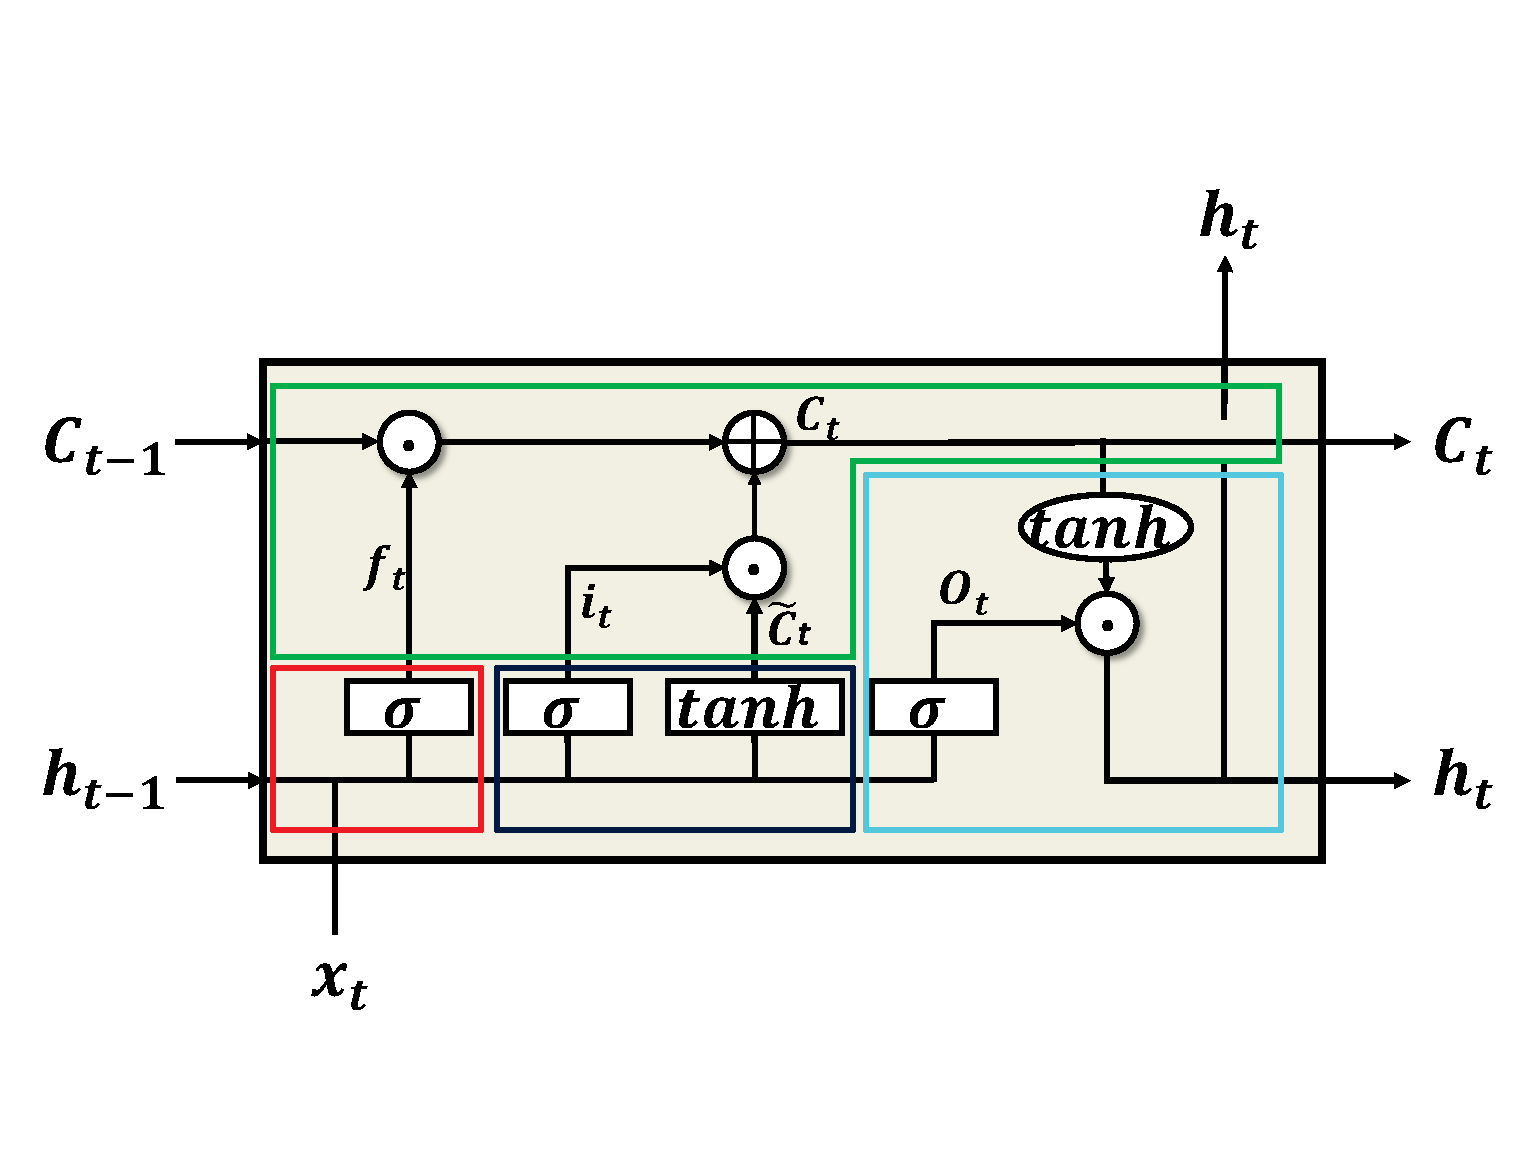
\includegraphics[width=.4\textwidth]{image/basic_LSTM_revised}
	\caption{Architecture of the LSTM. It consists of 3 gates, forget gate(the part inside the red box), input gate(the part inside the blue box), and output gate. And output gate is divided into cell state layer(the part inside the green box) and output gate layer(the part inside the cyan box) 
	}
	\label{fig:basic_lstm}
\end{figure}

Unlike RNN that consist only of hidden state, in LSTM, cell state is added on the network. The cell state consists of the 3 gates to preserve the previous information and control the cell state: forget gate, input gate, and output gate and equations of those are as follows:




\begin{align}
f_{t} & =\sigma _{s}\big(W_{xf}\cdot x_{t}+W_{hf}\cdot h_{t-1}+b_{f}\big)\label{eq:forget}\\
i_{t} & =\sigma _{s}\big(W_{xi}\cdot x_{t}+W_{hi}\cdot h_{t-1}+b_{i}\big)\label{eq:input}\\
\tilde{c}_{t} & = \tanh\big(W_{xc}\cdot x_{t}+W_{hc}\cdot h_{t-1}+b_{c}\big)\label{eq:new_cell}\\
c_{t} & =f_{t}\odot c_{t-1}+i_{t}\odot\tilde{c}_{t}\label{eq:update}\\
o_{t} & =\sigma _{s}\big(W_{xo}\cdot x_{t}+W_{ho}\cdot h_{t-1}+b_{o}\big)\label{eq:output}\\
h_{t} & =o_{t}\odot \tanh\big(c_{t}\big)\label{eq:hidden}
\end{align}

where $\sigma _{s}$ is a kind of activation function, called \textit{sigmoid},  $f_{t}$, $i_{t}$, and $o_{t}$ respectively indicates the forget gate, input gate, and output gates, and $c_{t}$ denotes cell states. And $\odot$ denotes element-wise multiplication, called \textit{Hadamard product}. Entire gates are activated by sigmoid function and cell states are activated by $\tanh$ function.

The Forget gate layer, $f_{t}$, decides how much information to forget. The sigmoid layer, which is the activation function of $f_{t}$, takes previous hidden state, $h_{t}$, and present input, $x_{t}$ and outputs a number between 0 and 1. Note that 1 indicates "totally keep the previous cell state, $C_{t-1}$" and 0 indicate "totally forget $C_{t-1}$" \eqref{eq:forget}. Next, the input gate, $i_{t}$, decides how much information to embrace when updating the cell state. $i_{t}$ are also from the sigmoid function layer \eqref{eq:input} and $tanh$ generates the new candidate cell state, $\tilde{c}_{t}$, which ranges from -1 to 1 \eqref{eq:new_cell}. After that, $c_{t}$ is updated by the cell state layer based on $f_{t}$, $i_{t}$, and $\tilde{c}_{t}$ \eqref{eq:update}. In addition, output gate layer, $o_{t}$, sereves as a filter, which means $o_{t}$ determine what values are going to output \eqref{eq:output} in such a way as that present hidden state, $h_{t}$, is updated based on $o_{t}$ updated cell state, $c_{t}$ \eqref{eq:hidden}. 


\subsection{Bidirectional LSTM}

\begin{figure}[h!]
	\centering
	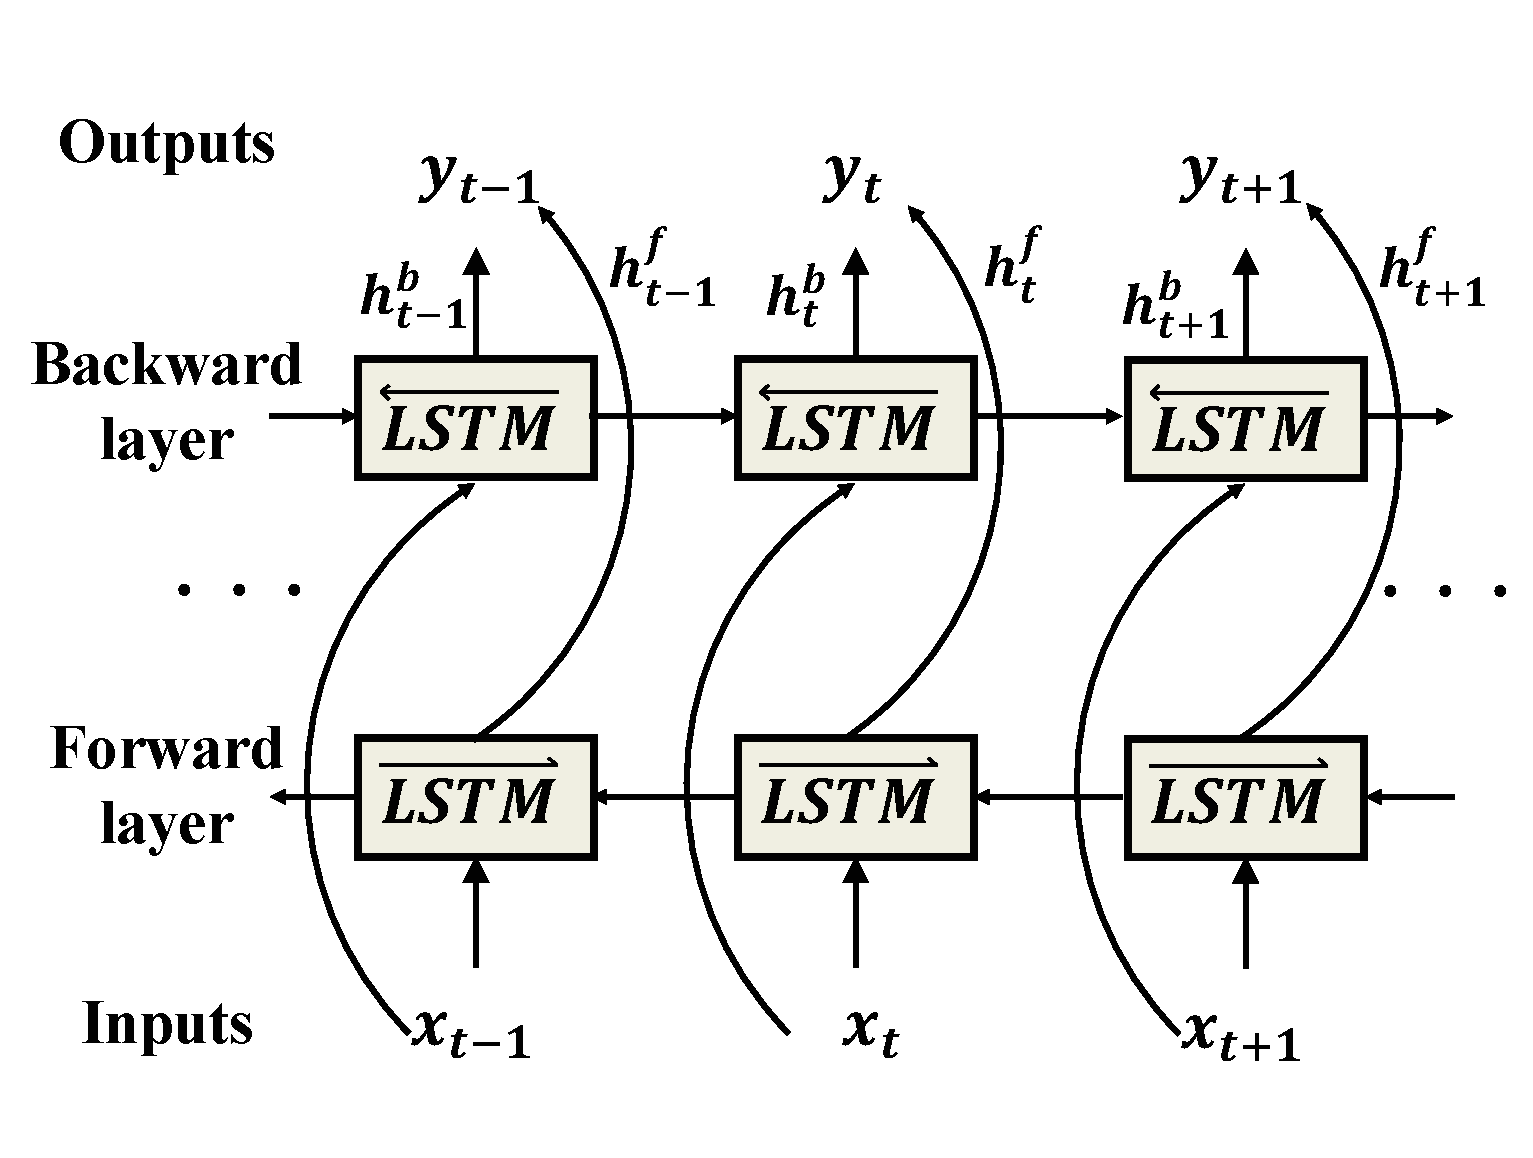
\includegraphics[width=.9\linewidth]{image/bidirectional_LSTM_revised}
	\caption{Architecture of the Bidirectional LSTM(Bi-LSTM)}
	\label{fig:bidirectional_revised}	
\end{figure}


One shortcoming of conventional RNNs is that they only exploit previous context to update $h_{t}$ and $c_{t}$. However, in many cases dealing with sequential data, it could be efficient to extract well-discribed context by utilizing future context as well. Bidirectional RNNs are introduced\cite{schuster1997bidirectional} for that reason and bidirectional RNNs process the data in both directions with two separate hidden layers. Especially, bidirectional LSTM, which we employee, has one forward LSTM and one backward LSTM running in reverse time and their features are combined at the output layer, $y_{t}$. As a result, bidirectional LSTM can produce more appropriate context considering both past and future at the same time. By virtue of this characteristics, bidirectional LSTM is popularly utilized for many tasks to model their sequentional systems \cite{zhang2017multi,li2018human,ullah2018action}. 


As FIGURE. \ref{fig:bidirectional_revised} shown, bidirectional LSTM consist of 2 LSTMs: one forward LSTM layer, $\overrightarrow{LSTM}$, and one backward LSTM layer, $\overleftarrow{LSTM}$. Let assume the hidden state of $\overrightarrow{LSTM}$ at the time step $t$  be $h^{f}_{t}$ and $\overleftarrow{LSTM}$ at the time step $t$  be $h^{b}_{t}$, the hidden states and output sequence, $y_{t}$ are calcaulated as follows:

\begin{align}
h^{f}_{t} & =\overrightarrow{LSTM}\big(x_{t}, h^{f}_{t-1}\big)\\
h^{b}_{t} & =\overleftarrow{LSTM}\big(x_{t}, h^{b}_{t+1}\big)\\
y_{t} & =\sigma _{R}\big(W_{h^{f}y}\cdot h^{f}_{t}+W_{h^{b}y}\cdot h^{b}_{t}+b_{y}\big)
\end{align}

where $\sigma _{R}$ denotes activation function called ReLu. Note that in our case, we concatenate $h^{f}_{t}$ and $h^{b}_{t}$ to preverse their contexts seperately as our range measurement, which is gathered by the tag node and each anchor node, suffer from the \textit{rank-dificiency},which means range-based measurement consist of one-dimensional data\cite{fabresse2013undelayed}. Hence, we judge that it would be more helpful to increase the number of features naturally by concatenating two hidden states rather than adding them and when the network infer the position  .

\subsection{Stacked Architecture}

Recently, researchers show that the deeper the architecture of neural networks, the better their performance\cite{simonyan2014very, he2016deep} and their demonstrations has opened a deep learning area. Likewise, many authors have analyzed variations of LSTM architecture and find out that stacking multiple layers of the LSTM improve the performance for many tasks\cite{graves2013hybrid, graves2013speech,ullah2018action}. In other words, as the number of stacked layers is getting large, the more activation functions which rise the non-linearity within the networks are stacked  in such a way as that complexity of networks increases. As a results, networks could model more complex system by virture of these increased non-linerity.

Therefore, we also construct our networks by stacking two LSTM to increase the non-linearity. Note that stacking more than three LSTM doesn't show the improvement of performance. We suppose that activation funtions within the LSTM cause the \textit{vanishing gradient problem}\cite{pascanu2013difficulty}, which the networks fail to training due to the fact that the gradient is getting closer to zero during the backpropagation. We deem that this problem could comes from the sigmoid function and $tanh$ function that compose the part of LSTM. Consequently, we put the ReLu function between LSTMs to avoid the vanishing gradient problem\cite{nair2010rectified}, instead of stacking LSTM.    


\subsection{Training loss}

In this section, we describe the method for training our network. Generally, let $n$ be the number of anchor nodes, data set measured by each anchor node and tag node are represented on the time step $t$ as follows:

\begin{equation}
L_{t} = (l_{1}, l_{2}, ..., l_{n})_{t}
\end{equation}

where $l_{i}$ denotes the the distance between $i^{th}$ anchor node and the tag node. Note that our neural network does not only take a set of distance data at the time $t$ but takes sets of distacne data based on the sequential length of input to our network, $T$. In other words, train data consist of $T$ sets of distance data  corresponding to the position of mobile nodes. Let $\mathbb{L}_t$ be 

\begin{equation}
%$L = \left\{(X_t, Y_t)\right \}$ 
\mathbb{L}_t = \left\{L_{t-T+1}, L_{t-T+2}, ..., L_t\right\} 
\end{equation}

Conseqeuntly, neural network  could be optimized to be able to localize the mobile node when take distance sets as input. Train data $\mathbb{D}$ are formulated as follows:

\begin{equation}
%$L = \left\{(X_t, Y_t)\right \}$ 
\mathbb{D} = {(\mathfrak{N}(\mathbb{L}_t), \mathfrak{N}(Y_t))} 
\end{equation}

where $Y_t$ denotes the ground truth of the robot's 2D position, which is denoted as $Y_t = (x_t, y_t)$ and $\mathfrak{N}$ denotes normalization function that transforms data to min-max scaling 0 to 1. Note that range measurements mesured by each range sensor are processed by each min-max scaling because each range sensor has own characteristic, as one calibrate range sensors respectively.  

Let $\Theta$ be the parameters of our network model and assume that the trained network model could be expressed as conditional probability as follows:

\begin{multline}
P(\mathfrak{N}(Y_t)|\mathfrak{N}(\mathbb{L}_t)) = p((x_t, y_t)|\left\{L_{t-T+1}, L_{t-T+2}, ..., L_t\right\})
\end{multline}  

Note that our approach takes sequential range data on the sequence length $T$ so that extract temporal features to map sets of the range measurements to position and also learn how to cover the noises and outliers, which temporarily caused by the MPF problem or unstable signal conditions. Then, our final goal is to find optimal parameters $\Theta^{*}$ for localization by minimizing $L_2$ loss term. The $L_2$ loss term indicates mean square error(MSE) of Euclidean distance between the normalized ground truth position $\mathfrak{N}(Y_k)$ and estimated position $\hat{Y_k}$ as follows:

\begin{equation}
\Theta^{*} = \underset{\Theta}{\mathrm{argmin}} \frac{1}{N} \sum_{k=1}^N \parallel \mathfrak{N}(Y_k) - \hat{Y_k} \parallel^{2}
\end{equation}  


\section{Experiments}
\subsection{Experimental environment}

Our experimental system consists of a UWB(ultra wideband) sensor tag node attached on the mobile robot platform and eight anchor nodes that have a UWB transceiver, the motion capture system with 12 cameras, and a SFF(small-form-factor) computer.

UWB sensor anchors are attached to landmarks. These become the end points of the range measurements. The anchor nodes transmit the UWB signal. A UWB sensor tag is attached to a robot. It becomes the opposite side end point of the measurements. The tag node receives the signal and measures the range between two devices. Each UWB transceiver, DW1000 UWB-chip made by Decawave, supports 6 RF bands from 3.5 GHz to 6.5 GHz. It measures in centimeter-level accuracy. Fig. \ref{fig:anchor_tag_nodes} shows our experimental environment briefly and how to the anchor nodes and the tag node are attatched.

\begin{figure}[h!]
	\centering
	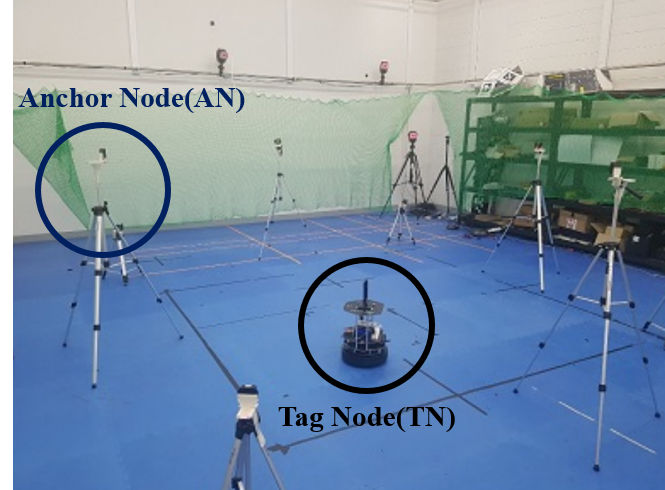
\includegraphics[width=.9\linewidth]{image/anchor_tag_nodes}
	\caption{our experimental environment briefly and how to the anchor nodes and the tag node are attatched.}
	\label{fig:anchor_tag_nodes}
\end{figure}

We inference the position of a robot with our network. To train the network and test the results, the ground truths are needed. We get the ground truth by using the motion capture system. The system is Eagle Digital Realtime system of motion analysis corporation that operates with the principle of stereo pattern recognition that is a kind of photogrammetry based on the epipolar geometry and the triangulation methodology. We attach four markers to a robot. The system gives us the location of these markers and has < 1mm accuracy.

A mobile robot used in experiment is iClebo Kobuki from Yujinrobot that has 70 cm/s maximum velocity.The SFF computer is a gigabyte Ultra compact PC. Deep learning framework used for our network is pytorch 0.4.0 on python 3.6. The network inferences on the same setting.

The UWB tag is attached to mobile robot that has a SFF computer. The UWB anchors are attached to stands that have two different heights. The anchors are positioned randomly in the square space where the motion capture system can measure the position. The robot moves in this sapce also. As you can see in Fig. \ref{fig:paths}, a mobile robot manually goes on various random trajectories by experimenters.

\begin{figure}[h!]
	\centering
	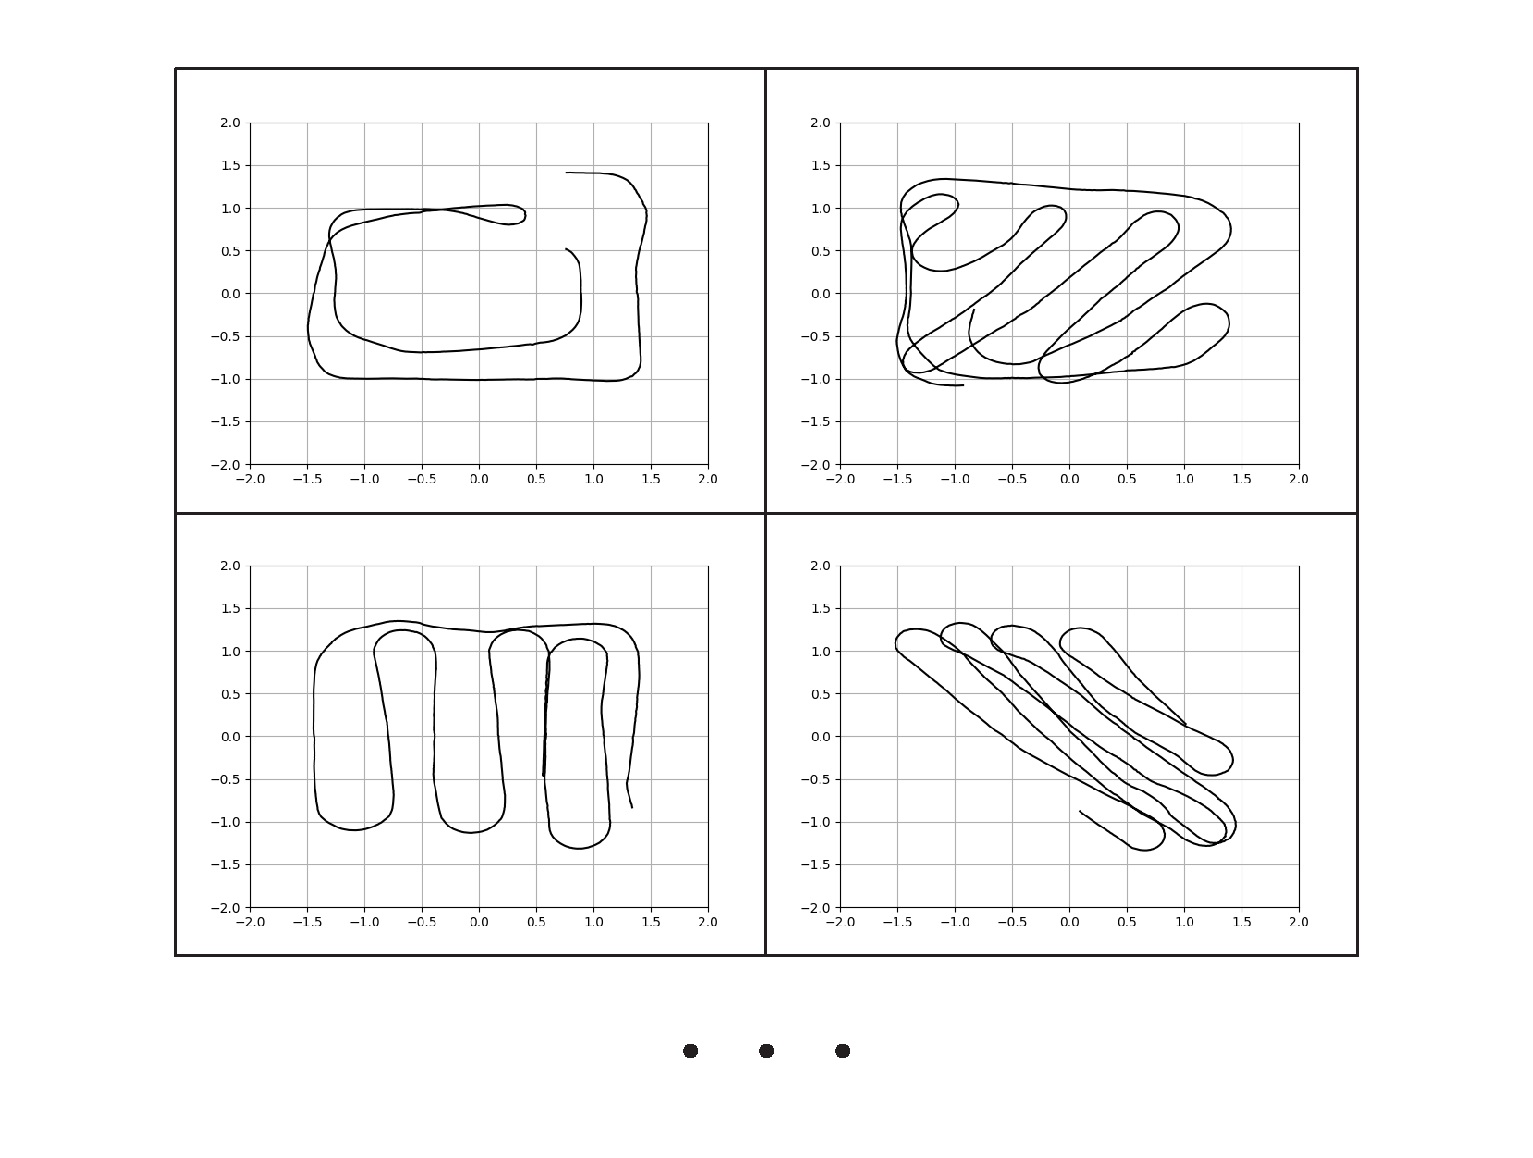
\includegraphics[width=0.9\linewidth]{image/paths_1}
	\caption{Four example of the trajectories}
	\label{fig:paths} 
\end{figure}

\subsection{Data syncronization for Train/Test data}
During the robot is going on, the data is saved in the computer. The distance data used for input data is measured by the UWB sensors. The global position data used for ground truth is measured by the motion capture system. These two kinds of data are paired in a dataset. Because these two data are transmitted by different frequency, we need to syncronize these. This process is conducted in a SFF computer. The computer receives these two kinds of data respectively and syncronizes these by time. To synchronize, we make an independent thread that concatenates and saves these data at the same time. The data is saved at 20Hz frequency. Each trajectory becomes one dataset. All the trajectories are different. Fig. \ref{fig:dataset} shows this process. After collecting whole datasets, we separate the entire dataset to two types, some are the training datasets and others are test datasets.

Ground truth data is robot's position measured by eagle eye motion capturer, whose error is in mm units.
\begin{figure}[h!]
	\centering
	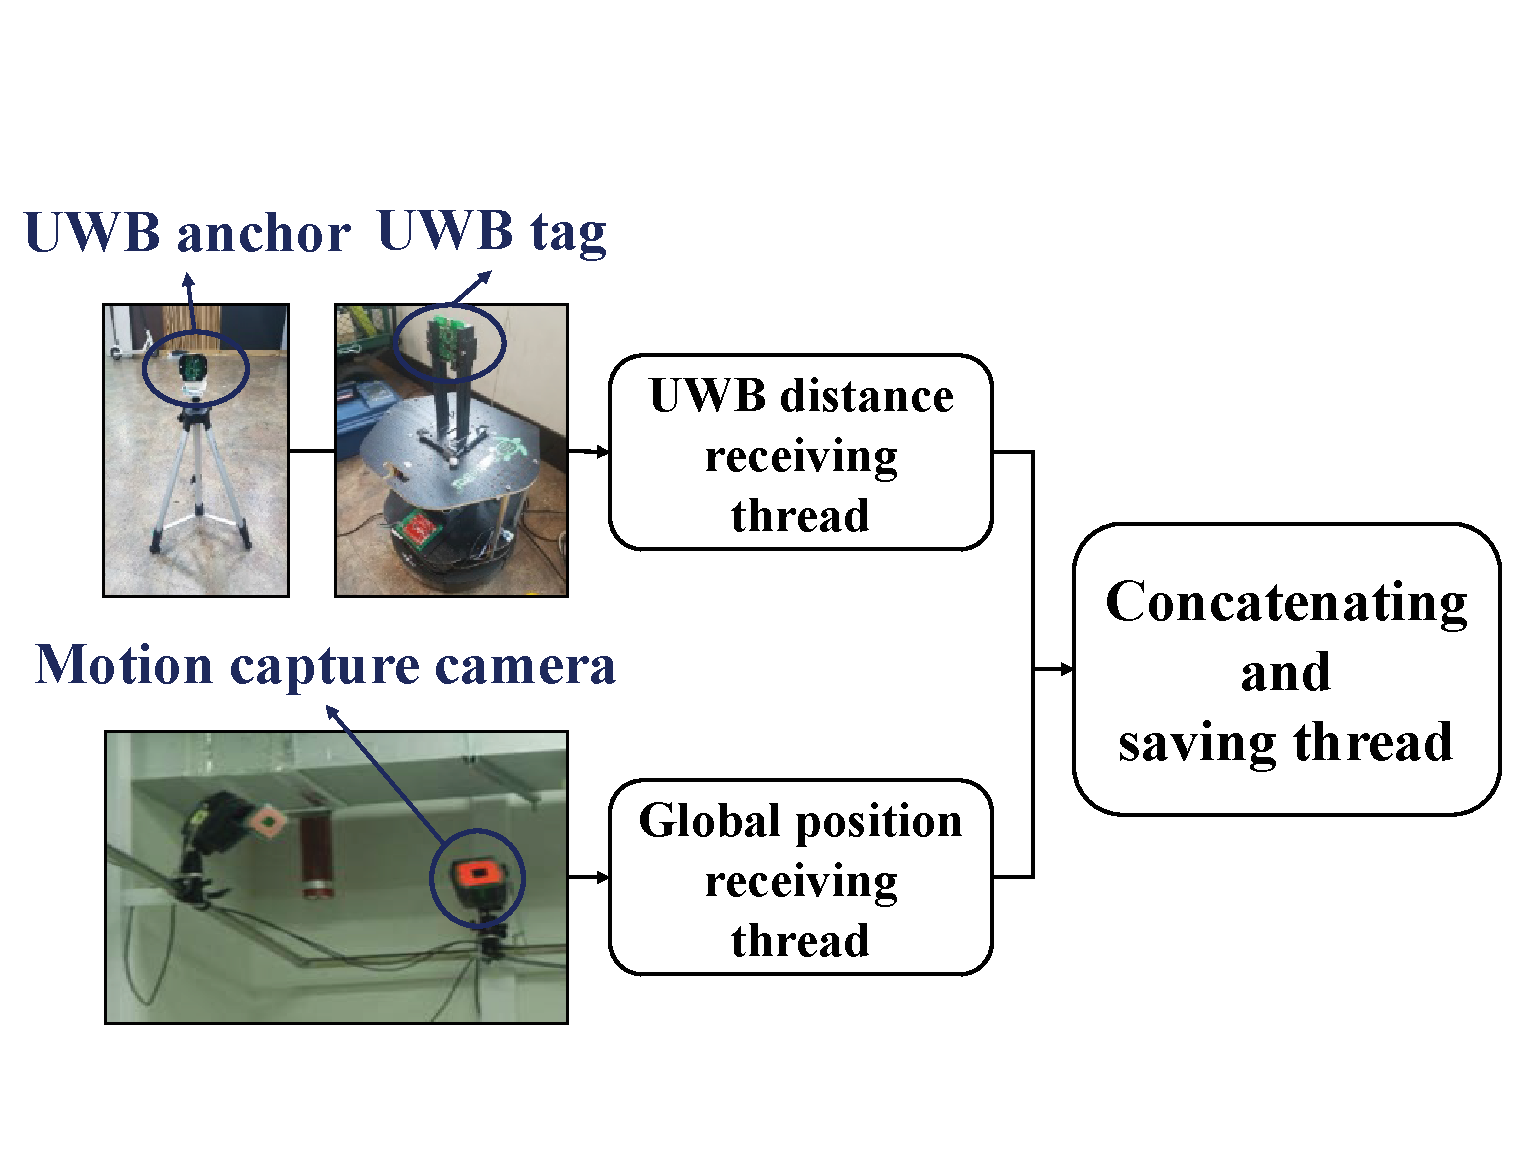
\includegraphics[width=0.9\linewidth]{image/data_sync}
	\caption{the process that makes dataset}
	\label{fig:dataset} 	
\end{figure}

\subsection{Training the Networks}

Pass

\section{Results}

To improve the performance of our proposed networks, we check which seqeunce length is optimal for localization of MN. And then, we implemented and trained other previous networks to compare their performance when our real-world data are given as input. We set three test trajectory cases: a square path, a verical and horizontal winding path, and a diagonal winding path. 

\subsection{Performance according to the sequence length}

Even though LSTM solve the long term dependency problem, we thought that it would not always make neural network perform better as sequence length become more longer. So, as part of turning hyperparameters, we modified sequence length of our network in a variety of numbers to find optimal sequence length.   

As illustrated in FIGURE. \ref{fig:paths}, The train data are gathered by the robot that arbitrary moves on the region where the motion capture camera cover. The neural network takes distances measured by each AN and a MN as input and outputs robot's position. The Root-Mean-Squared Error (RMSE) results of trajectory prediction with respect to sequence length are shown in FIGURE. \ref{fig:seq_length} and specific figures are shown in Table \ref{table:RMSE_sequence}.

As a result, we found that there is a trade-off between robustness and improvement of general performance according to the sequence length. Figure. \ref{fig:seq_length} show that as longer the sequence length, as more inaccurate the mean performance. This is because it is hard for the neural architecture to train the chracteristics of the sequential data. In other words, as sequence length become longer, the tendency of the values may be different due to accumulation of different patterns of system noises even if the data is acquired by moving to a similar path in the train data. Note that network with longer sequence length tend to have less error variance and more a ability to generalize the situation since they could utilize more extended temporal information. By doing so, the nerual network have the ability to suppress the disturbance caused by noises.

Similarily, as sequence length become shorter, it is less difficult for the neural architecture to understand the chracteristics of the sequential data by virtue of the less accumulation of different patterns of system noises. Note that in most cases, the network constructed by the shorter sequential length tend to estimate the position more precisely than those with longer sequential lengths. However, it becomes a double-edged sword because temporal information is also reduced accordingly in such a way as to week to the noises, having larger error variance.



%sequence length가 길어질수록 netowrk가 그 sequential data를 일반화 시키는 게 어렵다
%In other workds, sequence length만큼 끊어서 input으로 받기 때문에 sequential한 경향성에 대해 적절한 output을 내게 학습을 하는데, sequence가 길어지게 되면 길어지는 만큼 그 상황이 특수해져서 비슷한 특성을 지닌 input이 줄기 때문이다????
%길이가 길어짐에 따라 noise에 대한 방해를 더 길어진 temporal information을 활용해서 억누를 수 있다.
%On the other hand, 짧아질수록 좋지만 경향성을 학습?


\begin{figure}[h!]
	\centering
	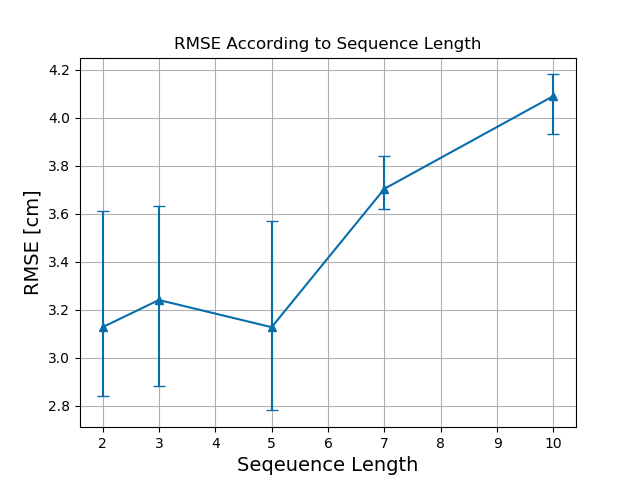
\includegraphics[width=0.9\linewidth]{image/seq_result_prototype}
	\caption{Error bar graph of RMSE with respect to sequence length}
	\label{fig:seq_length} 	
\end{figure}


\begin{table}[h]
	\centering
	\caption{Root mean squared error of each case}
	\begin{tabular}{clllll}
		\toprule
		\multicolumn{6}{c}{The results of RMSE[cm]}                         \\
		\midrule
		& \multicolumn{5}{c}{Sequence length} \\  \cmidrule{2-6}
		
		\multicolumn{1}{l}{} & 2     & 3       & 5      & 7    & 10  \\
		Test1                & 2.84  & 2.88    & \textbf{2.78}   & 3.65 & 4.16 \\
		Test2                & 3.61  & 3.63    & \textbf{3.57}   & 3.84 & 4.18 \\
		Test3                & \textbf{2.93}  & 3.21    & 3.03   & 3.62 & 3.93 \\
		\bottomrule 
		
	\end{tabular}
	\label{table:RMSE_sequence}
\end{table}

\subsection{Performance comparison result}

The results of trajectory prediction are shown in Fig. 3(a) and Fig. 3(d) and
Root-Mean-Squared Error (RMSE) are shown in Table 1. Performance is better
in order of stacked Bi-LSTM, Bi-LSTM, LSTM and GRU. In case of GRU, it
has only two gates which is less complex structure than LSTM [27]. However,
due to GRU's less complexity, GRU has less number of neurons than LSTM so
their non-linear mapping achieves less performance. Likewise, Bi-LSTM consists
of two LSTMs to process sequence in two directions so that infer output using
the correlation of the backward information and the forward information of the
sequences of each time step with its two separate hidden layers. Thus, Bi-LSTM
has better nonlinear mapping capability than LSTM. For similar reasons, stacked
Bi-LSTM is the architecture that stacks two Bi-LSTMs, so inference performance
is better than Bi-LSTM. As a result, the stacked Bi-LSTM showed the best
performance among unit RNN architectures. Therefore, we can conclude that
the performance improves as the non-linearity of the architecture increases.


!!!!!!!!!!!!!!!!!
We also verified effectiveness of attention layer. It was confirmed that the performance of the networks with the attention layer is improved compared to the networks without the attention layer.
We also provide statistical analysis from simulations demonstrating that
our new approach can cope with highly noisy sensors and
reduces in one order of magnitude the average errors of the
method proposed
!!!!!!!!!!!!!!!!!


\section{Conclusion}

In this paper, we proposed a novel approach to range-only SLAM using multimodal-based RNN models and tested our architectures in two test data.

Using deep learning, our structure directly learns the end-to-end mapping between distance data and robot position. The multimodal bidirectional stacked LSTM structure exhibits the precise estimates of robot positions. We set two test trajectory cases: an square path and zigzag path. an The results shows that it has better performance than established probabilistic-based approach. In both cases, performance of our networks  is better that of particle filter. RMSE of our networks in test1 is 3.928cm and 4.119cm in test2. Therefore, we could check the possibility that our multimodal LSTM-based structure can substitute traditional algorithms

As a future work, because we conducted on just localization, this approach may not be operated when locations of sensors are changed. Therefore, the proposed method needs to be revised for precise estimates even though locations of anchors are changed. 
\bibliographystyle{IEEEtran}
% argument is your BibTeX string definitions and bibliography database(s)
\bibliography{./IEEEabrv,./IROS_RObib}


\end{document}
